\documentclass[a4paper,12pt,oneside, tikz]{book}  
\usepackage[utf8]{inputenc}
\usepackage{tcolorbox}
\usepackage{amsmath,amssymb,amsthm, enumitem, hyperref, tabto} 
\usepackage[T1]{fontenc}
\usepackage[utf8]{inputenc}
\usepackage[english]{babel}
\usepackage{wrapfig}
\usepackage{lastpage}
\usepackage{tikz}
\usetikzlibrary{external}
\tikzexternalize % activate!
\usepackage[american]{circuitikz}
\usepackage[absolute,overlay]{textpos}
\usepackage[left=2cm,right=2cm]{geometry}
\usepackage[english]{babel}
\usepackage{fancyhdr}
\usepackage{float}
\hypersetup{
    colorlinks=true,
    linkcolor=blue,
    filecolor=magenta,      
    urlcolor=cyan,
    pdftitle={Studio 4},
    pdfpagemode=FullScreen,
    }

\urlstyle{same}
\usepackage{xcolor}
\usepackage{colortbl}

\usepackage{graphicx, multicol, latexsym}
\usepackage{blindtext}
\usepackage{subfigure}
\usepackage{caption}
\usepackage{capt-of}
\usepackage{tabu}
\usepackage{booktabs}

\usepackage{fancyhdr}            % Permits header customization. See header section below.
\fancypagestyle{plain}{
    \lhead{}
    \fancyhead[R]{\thepage}
    \fancyhead[L]{}
    \renewcommand{\headrulewidth}{0pt}
    \fancyfoot{}
}

\pagestyle{fancy}
\fancyhead[R]{\thepage}
\fancyhead[L]{}
\renewcommand{\headrulewidth}{0pt}
\fancyfoot{}

\usepackage{array}
\newcolumntype{P}[1]{>{\centering\arraybackslash}p{#1}}

\usepackage{titlesec}

\titleformat{\chapter}[display]{\normalfont\huge\bfseries}{\chaptertitlename\ \thechapter}{20pt}{\Huge}

% this alters "before" spacing (the second length argument) to 0
\titlespacing*{\chapter}{0pt}{0pt}{40pt}


\addto\captionsenglish{\renewcommand{\chaptername}{Activity}} 


\title{\textbf{Basic Op-Amps} Studio Report \\ CG1111A Studio 8}

\author{Prannaya Gupta (B02)}

\begin{document}

\maketitle

\chapter{Non-Inverting Op-Amp}

\section{Derive the Gain Relationship}
\begin{tcolorbox}
Let $I_\text{in}$ and $I_\text{out}$ be the input and output currents respectively.

\begin{align*}
    I_\text{out} &= \frac{V_\text{out}}{R_f + R_\text{in}} \\
    V^- &= I_\text{out} R_\text{in} = V_\text{out} \left(1 + \frac{R_f}{R_\text{in}} \right)^{-1} \\
    V_\text{out} &= A(V^+ - V^-) \\
    \frac{V_\text{out}}{A} &= V_\text{in} - V_\text{out} \left(1 + \frac{R_f}{R_\text{in}} \right)^{-1} \\
    \text{In ideal circumstances, }&\text{A is very large, thus LHS is 0} \\
    V_\text{out} \left(1 + \frac{R_f}{R_\text{in}} \right)^{-1} &= V_\text{in} \\
    V_\text{out} &= V_\text{in}\left(1 + \frac{R_f}{R_\text{in}} \right)
\end{align*}
\end{tcolorbox}

\section{Experimental Data}
As measured, $V_\text{in} = 0.20525$ V.

\begin{table}[H]
    \centering
    \begin{tabular}{|c|c|c|c|c|}
        \hline S/N & $R_f$ (k$\Omega$) & $R_\text{in}$ (k$\Omega$) & $\text{Gain} = V_\text{out} / V_\text{in}$ & $V_\text{out}$ (V) \\
        \hline 1 & 10 & 10 & 2 & 0.40505 \\
               2 & 33 & 10 & 4.3 & 0.88977 \\
               3 & 100 & 10 & 11 & 2.2311 \\
               4 & 220 & 10 & 23 & 4.6813 \\
               5 & 1000 & 10 & 101 & 8.7118  \\
        \hline
    \end{tabular}
    \caption{Table of Results for Activity 1}
    \label{tab:act1}
\end{table}

\section{Results Analysis}
\begin{tcolorbox}
\textbf{Q1. Is the output voltage measured from the oscilloscope like what you have computed from the derived gain relationship of the op amp from Step 1? Explain your observations.} \\

For the first four readings, it is about the same. To compare, here is a table of comparison:

\begin{center}
    \begin{tabular}{|c|c|}
 \hline Calculated & Measured \\
 \hline 0.41050 & 0.40505 \\
        0.882575 & 0.88977 \\
        2.25775 & 2.2311 \\
        4.72075 & 4.6813 \\
 \hline
    \end{tabular}
\end{center}

For the fifth reading, explanation is in the third question.

As for the rest, the readings grow approximately proportionally based off the gain, with some error.

This essentially proves that the operational amplifier is in fact doing its job by amplifying the signal.
\end{tcolorbox}
\begin{tcolorbox}
\textbf{Q2. Is the output voltage in-phase with the input voltage signal?} \\
Yes, as observed:
\begin{figure}[H]
    \centering
    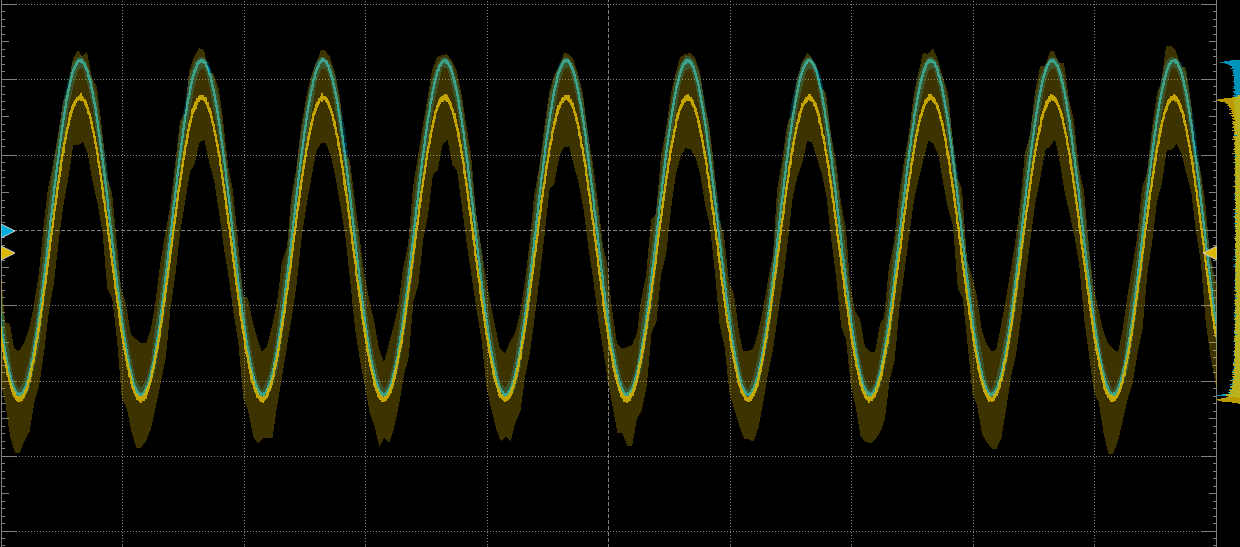
\includegraphics[width=120mm]{./images/in_phase.png}
\end{figure}
\end{tcolorbox}
\begin{tcolorbox}
\textbf{Q3. What can you observe about the 5th combination of resistances? Why do you think this occurs?} \\
There is an observed plateau in the wave, as shown below:
\begin{figure}[H]
    \centering
    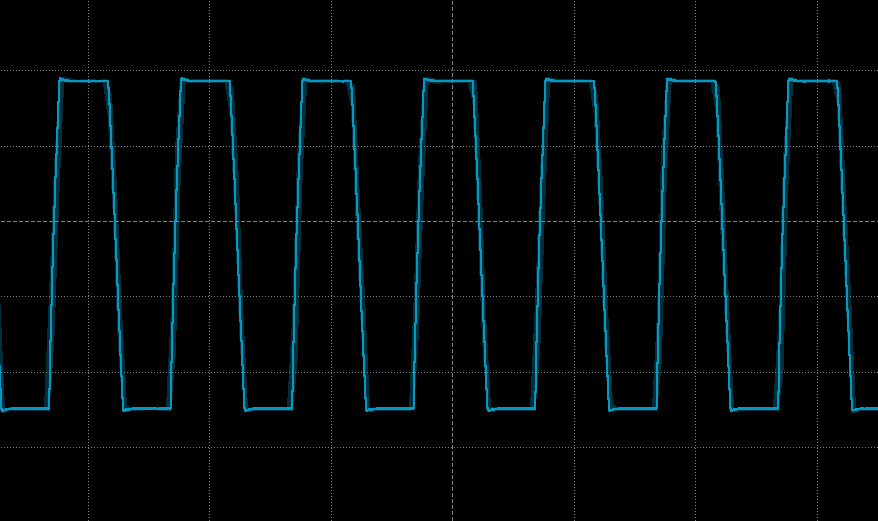
\includegraphics[width=120mm]{./images/plateau.png}
\end{figure}

The reason for this could be the fact that the operational amplifier reaches it's saturation value and this causes it to stop at that value instead of proceeding to the ideal value ($V_\text{out} = 20.73025$ V). Thus, observed is a plateau until such time that $V_\text{out}$ reduces to below $V_\text{sat}$.

\end{tcolorbox}


\chapter{Inverting Op-Amp}

\section{Derive the Gain Relationship (Challenge Yourself)}
\begin{tcolorbox}
Let $I_\text{in}$ and $I_\text{out}$ be the input and output currents respectively.
\begin{align*}
    V^- &= I_\text{out}R_f + V_\text{out} \\
    V^- &= V_\text{in} - I_\text{in} R_\text{in} \\
    V_\text{out} &= A \left(V^+ - V^- \right) = -AV^- \\
    \text{Note that }I_\text{in} &= I_\text{out}. \\
    \frac{V^- - V_\text{out}}{R_f} &= \frac{V_\text{in} - V^-}{R_\text{in}} \\
    R_\text{in} (V^- - V_\text{out}) &= R_f (V_\text{in} - V^-) \\
    V_\text{out} R_\text{in} &= -\frac{V_\text{out}}{A}(R_\text{in} + R_f) - V_\text{in} R_f \\
    V_\text{out} &= -V_\text{in} \frac{R_f}{R_\text{in}}
\end{align*}

Apologies if this is wrong. We spent quite a bit of time thinking about it but we weren't able to come up with a solution that doesn't approximate $A$ to $\infty$.
\end{tcolorbox}

\section{Experimental Data}
As measured, $V_\text{in} = 0.20452$ V.

\begin{table}[H]
    \centering
    \begin{tabular}{|c|c|c|c|c|}
        \hline S/N & $R_f$ (k$\Omega$) & $R_\text{in}$ (k$\Omega$) & $\text{Gain} = V_\text{out} / V_\text{in}$ & $V_\text{out}$ (V) \\
        \hline 1 & 10 & 10 & -1 & 0.20252 \\
               2 & 33 & 10 & -3.3 & 0.68393 \\
               3 & 100 & 10 & -10 & 2.0784 \\
               4 & 220 & 10 & -22 & 4.4887 \\
               5 & 1000 & 10 & -100 & 8.6587 \\
        \hline
    \end{tabular}
    \caption{Table of Results for Activity 2}
    \label{tab:act2}
\end{table}



\section{Results Analysis}
\begin{tcolorbox}
\textbf{Q1. Is the output voltage measured from the oscilloscope like what you have computed from the derived gain relationship of the op amp from Step 1? Explain your observations.} \\

For the first four readings, it is about the same. To compare, here is a table of comparison:

\begin{center}
    \begin{tabular}{|c|c|}
 \hline Calculated & Measured \\
 \hline 0.20452 & 0.20252 \\
        0.674916 & 0.68393 \\
        2.0452 & 2.0784 \\
        4.49944 & 4.4887 \\
 \hline
    \end{tabular}
\end{center}

For the fifth reading, explanation is in the third question.

As for the rest, the readings grow approximately proportionally based off the gain, with some error.

This essentially proves that the operational amplifier is in fact doing its job by amplifying the signal.
\end{tcolorbox}
\begin{tcolorbox}
\textbf{Q2. Is the output voltage in-phase with the input voltage signal?} \\
No, it is 180${}^\circ$ out of phase. as observed:
\begin{figure}[H]
    \centering
    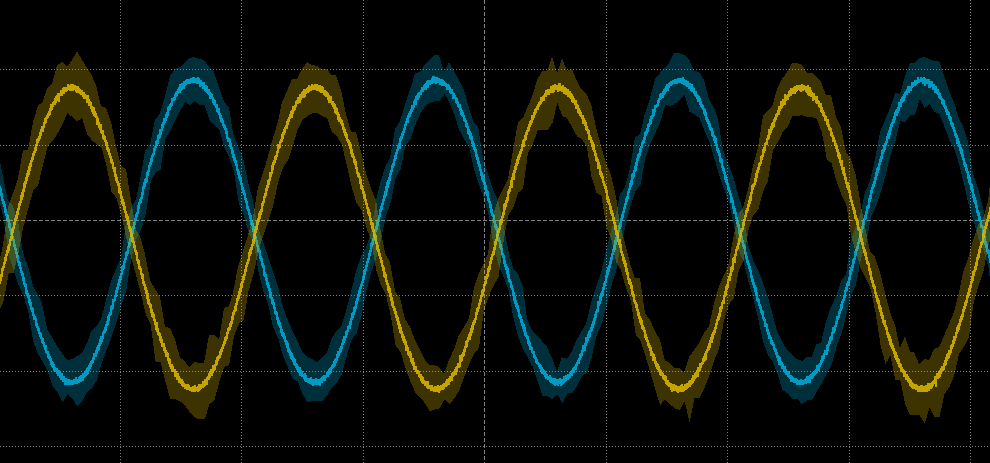
\includegraphics[width=120mm]{./images/out_phase.png}
\end{figure}

\end{tcolorbox}\begin{tcolorbox}
\textbf{Q3. What can you observe about the 5th combination of resistances? Why do you think this occurs?} \\
There is an observed plateau in the wave, as shown below:
\begin{figure}[H]
    \centering
    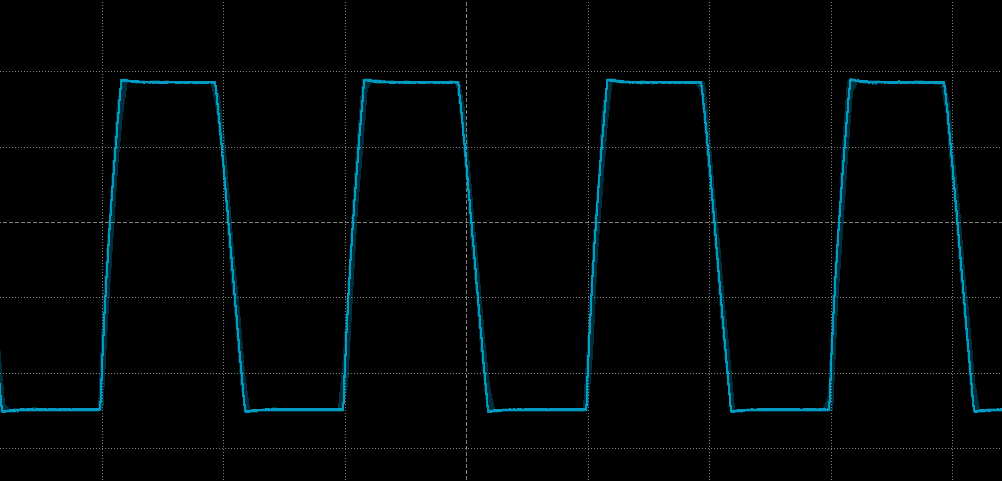
\includegraphics[width=120mm]{./images/plateau2.png}
\end{figure}

The reason for this could be the fact that the operational amplifier reaches it's saturation value and this causes it to stop at that value instead of proceeding to the ideal value ($V_\text{out} = 20.452$ V). Thus, observed is a plateau until such time that $V_\text{out}$ reduces to below $V_\text{sat}$.

\end{tcolorbox}

\end{document}